
\section*{Solutions to Exercises from Section 6}

\begin{solution}\label{sol:6.1}\ref{ex:6.1}
    \begin{enumerate}
        \item $A^{\complement}=\{ 0,2,5,8,10 \}$
        \item $B^{\complement}=\{ 0,1,2,3,7,9,10 \}$
        \item $A\cap A^{\complement}=\{ 0,2,5,8,10 \}\cap \{ 4,3,6,7,1,9 \}=\varnothing$
        \item $A\cup A^{\complement}=U$ by the same logic as the above example
        \item $A-A^{\complement}=\{ 0,2,5,8,10 \}-\{ 4,3,6,7,1,9 \}=\{ 0,2,5,8,10 \}=A$
        \item $A-B^{\complement}=\{ 4,6 \}$
        \item $A^{\complement}-B^{\complement}=\{ 5,8 \}$
        \item $A^{\complement}\cap B=\{ 5,8 \}$
        \item ${(A^{\complement}-B)}^{\complement}=\{ 1,3,4,5,6,7,9 \}$
    \end{enumerate}
\end{solution}

\begin{solution}\label{sol:6.2}\ref{ex:6.2}
    \begin{enumerate}
        \item $A^{\complement}=\{ 1,3,5,7 \}=B$
        \item $B^{\complement}=\{ 0,2,4,6,8 \}=A$
        \item $A\cap A^{\complement}=\varnothing$
        \item $A\cup A^{\complement}=U$
        \item $A-A^{\complement}=A$
        \item ${(A\cup B)}^{\complement}=\varnothing$
        \item $A^\complement\cap B^{\complement}=\varnothing$
        \item ${(A\cap B)}^{\complement}=U$
        \item $A^{\complement}\times B=\{ (1,1),(1,3),(1,5),\dots \}=B^{2}$
    \end{enumerate}
\end{solution}

\begin{solution}\label{sol:6.3}\ref{ex:6.3}
    You can find the solution for this exercise below. 
    \begin{figure}[htbp]
    \centering
    % Drawing 1: The set X
    \begin{subfigure}[b]{0.32\linewidth}
        \centering
        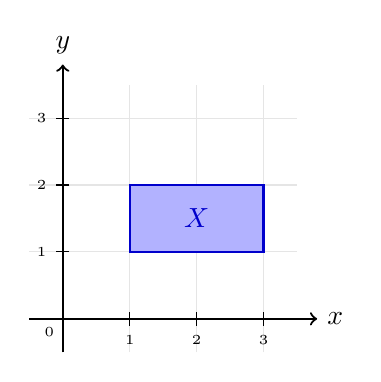
\begin{tikzpicture}[scale=0.85]
            % Grid & Axes
            \draw[gray!20, thin] (-0.5,-0.5) grid (3.5,3.5);
            \draw[->, thick] (-0.5,0) -- (3.8,0) node[right] {$x$};
            \draw[->, thick] (0,-0.5) -- (0,3.8) node[above] {$y$};
            
            % Ticks
            \foreach \x in {1,2,3} \draw (\x,0.1) -- (\x,-0.1) node[below] {\tiny $\x$};
            \foreach \y in {1,2,3} \draw (0.1,\y) -- (-0.1,\y) node[left] {\tiny $\y$};
            \node at (-0.2,-0.2) {\tiny $0$};

            % Set X: Shaded rectangle [1,3] x [1,2]
            \fill[blue!30] (1,1) rectangle (3,2);
            \draw[thick, blue!80!black] (1,1) rectangle (3,2);
            
            \node[blue!80!black] at (2,1.5) {$X$};
        \end{tikzpicture}
        \caption{The set $X = [1,3]\times[1,2]$}
    \end{subfigure}\hfill
    % Drawing 2: The set X^c
    \begin{subfigure}[b]{0.32\linewidth}
        \centering
        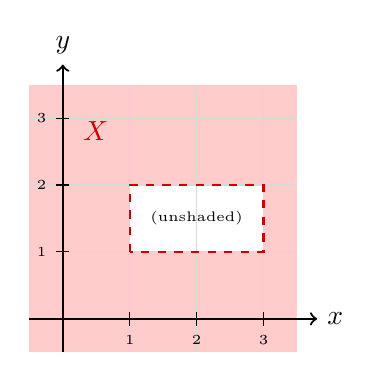
\begin{tikzpicture}[scale=0.85]
            % Outer shaded plane bounding box
            \fill[red!20] (-0.5,-0.5) rectangle (3.5,3.5);
            
            % Unshade the "hole" X
            \fill[white] (1,1) rectangle (3,2);
            
            % Grid & Axes
            \draw[gray!30, thin] (-0.5,-0.5) grid (3.5,3.5);
            \draw[->, thick] (-0.5,0) -- (3.8,0) node[right] {$x$};
            \draw[->, thick] (0,-0.5) -- (0,3.8) node[above] {$y$};
            
            % Ticks
            \foreach \x in {1,2,3} \draw (\x,0.1) -- (\x,-0.1) node[below] {\tiny $\x$};
            \foreach \y in {1,2,3} \draw (0.1,\y) -- (-0.1,\y) node[left] {\tiny $\y$};
            
            % Boundary of hole X
            \draw[thick, dashed, red!80!black] (1,1) rectangle (3,2);
            
            \node[red!80!black] at (0.5,2.8) {$X^{\complement}$};
            \node at (2,1.5) {\tiny (unshaded)};
        \end{tikzpicture}
        \caption{The complement $X^{\complement}$}
    \end{subfigure}\hfill
    % Drawing 3: X^c \cap ([0,2] \times [0,3])
    \begin{subfigure}[b]{0.32\linewidth}
        \centering
        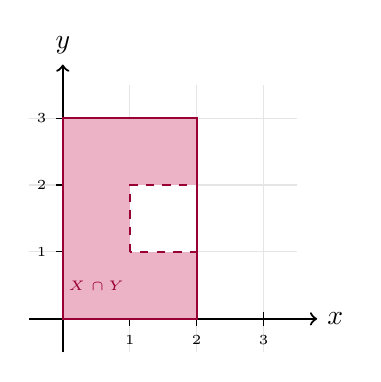
\begin{tikzpicture}[scale=0.85]
            % Grid & Axes
            \draw[gray!20, thin] (-0.5,-0.5) grid (3.5,3.5);
            \draw[->, thick] (-0.5,0) -- (3.8,0) node[right] {$x$};
            \draw[->, thick] (0,-0.5) -- (0,3.8) node[above] {$y$};
            
            % Ticks
            \foreach \x in {1,2,3} \draw (\x,0.1) -- (\x,-0.1) node[below] {\tiny $\x$};
            \foreach \y in {1,2,3} \draw (0.1,\y) -- (-0.1,\y) node[left] {\tiny $\y$};
            
            % Full region [0,2] x [0,3] shaded
            \fill[purple!30] (0,0) rectangle (2,3);
            % Hole where X overlaps: [1,2] x [1,2]
            \fill[white] (1,1) rectangle (2,2);
            
            % Outer boundary of [0,2] x [0,3]
            \draw[thick, purple!80!black] (0,0) rectangle (2,3);
            % Boundary of the removed hole
            \draw[thick, dashed, purple!80!black] (1,1) rectangle (2,2);
            
            \node[purple!80!black, font=\tiny] at (0.5,0.5) {$X^{\complement} \cap Y$};
        \end{tikzpicture}
        \caption{$X^{\complement}\cap([0,2]\times[0,3])$}
    \end{subfigure}

    \caption{Sketches of $X$, its complement $X^{\complement}$, and the restricted intersection.}\label{fig:ex_6_3}
\end{figure}
\end{solution}

\begin{solution}\label{sol:6.4}\ref{ex:6.4}
    Ditto.

    \begin{figure}[htbp]
    \centering
    % Drawing 1: The set X
    \begin{subfigure}[b]{0.32\linewidth}
        \centering
        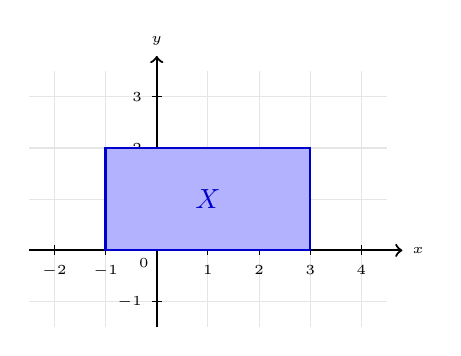
\begin{tikzpicture}[scale=0.65]
            % Grid & Axes
            \draw[gray!20, thin] (-2.5,-1.5) grid (4.5,3.5);
            \draw[->, thick] (-2.5,0) -- (4.8,0) node[right] {\tiny $x$};
            \draw[->, thick] (0,-1.5) -- (0,3.8) node[above] {\tiny $y$};
            
            % Ticks
            \foreach \x in {-2,-1,1,2,3,4} \draw (\x,0.1) -- (\x,-0.1) node[below] {\tiny $\x$};
            \foreach \y in {-1,1,2,3} \draw (0.1,\y) -- (-0.1,\y) node[left] {\tiny $\y$};
            \node at (-0.25,-0.25) {\tiny $0$};

            % Set X: Shaded rectangle [-1,3] x [0,2]
            \fill[blue!30] (-1,0) rectangle (3,2);
            \draw[thick, blue!80!black] (-1,0) rectangle (3,2);
            
            \node[blue!80!black] at (1,1) {$X$};
        \end{tikzpicture}
        \caption{The set $X$}
    \end{subfigure}\hfill
    % Drawing 2: The set X^c
    \begin{subfigure}[b]{0.32\linewidth}
        \centering
        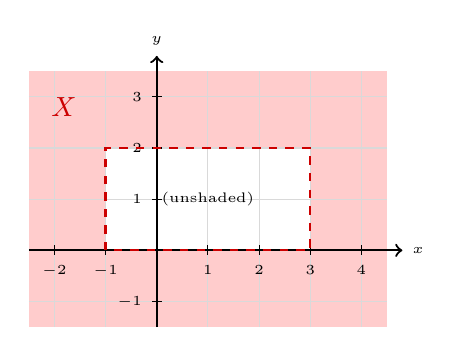
\begin{tikzpicture}[scale=0.65]
            % Outer shaded plane bounding box
            \fill[red!20] (-2.5,-1.5) rectangle (4.5,3.5);
            
            % Unshade the "hole" X
            \fill[white] (-1,0) rectangle (3,2);
            
            % Grid & Axes
            \draw[gray!30, thin] (-2.5,-1.5) grid (4.5,3.5);
            \draw[->, thick] (-2.5,0) -- (4.8,0) node[right] {\tiny $x$};
            \draw[->, thick] (0,-1.5) -- (0,3.8) node[above] {\tiny $y$};
            
            % Ticks
            \foreach \x in {-2,-1,1,2,3,4} \draw (\x,0.1) -- (\x,-0.1) node[below] {\tiny $\x$};
            \foreach \y in {-1,1,2,3} \draw (0.1,\y) -- (-0.1,\y) node[left] {\tiny $\y$};
            
            % Boundary of hole X
            \draw[thick, dashed, red!80!black] (-1,0) rectangle (3,2);
            
            \node[red!80!black] at (-1.8,2.8) {$X^{\complement}$};
            \node at (1,1) {\tiny (unshaded)};
        \end{tikzpicture}
        \caption{The complement $X^{\complement}$}
    \end{subfigure}\hfill
    % Drawing 3: X^c \cap ([-2,4] \times [-1,3])
    \begin{subfigure}[b]{0.32\linewidth}
        \centering
        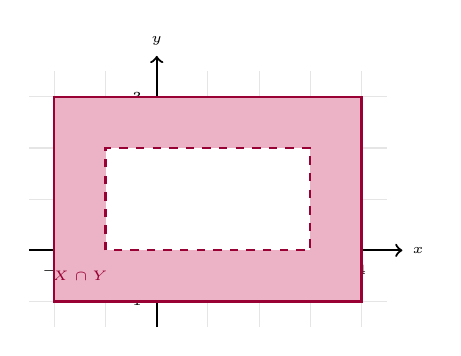
\begin{tikzpicture}[scale=0.65]
            % Grid & Axes
            \draw[gray!20, thin] (-2.5,-1.5) grid (4.5,3.5);
            \draw[->, thick] (-2.5,0) -- (4.8,0) node[right] {\tiny $x$};
            \draw[->, thick] (0,-1.5) -- (0,3.8) node[above] {\tiny $y$};
            
            % Ticks
            \foreach \x in {-2,-1,1,2,3,4} \draw (\x,0.1) -- (\x,-0.1) node[below] {\tiny $\x$};
            \foreach \y in {-1,1,2,3} \draw (0.1,\y) -- (-0.1,\y) node[left] {\tiny $\y$};
            
            % Full region [-2,4] x [-1,3] shaded
            \fill[purple!30] (-2,-1) rectangle (4,3);
            % Hole where X overlaps: [-1,3] x [0,2]
            \fill[white] (-1,0) rectangle (3,2);
            
            % Outer boundary of [-2,4] x [-1,3]
            \draw[thick, purple!80!black] (-2,-1) rectangle (4,3);
            % Boundary of the removed hole
            \draw[thick, dashed, purple!80!black] (-1,0) rectangle (3,2);
            
            \node[purple!80!black, font=\tiny] at (-1.5,-0.5) {$X^{\complement} \cap Y$};
        \end{tikzpicture}
        \caption{$X^{\complement}\cap([-2,4]\times[-1,3])$}
    \end{subfigure}

    \caption{Sketches for Exercise 6.4.}\label{fig:ex_6_4}
\end{figure}
\end{solution}

\begin{solution}\label{sol:6.5}\ref{ex:6.5}
    Ditto.
    \begin{figure}[htbp]
    \centering
    % Drawing 1: The set X (Annulus)
    \begin{subfigure}[b]{0.45\linewidth}
        \centering
        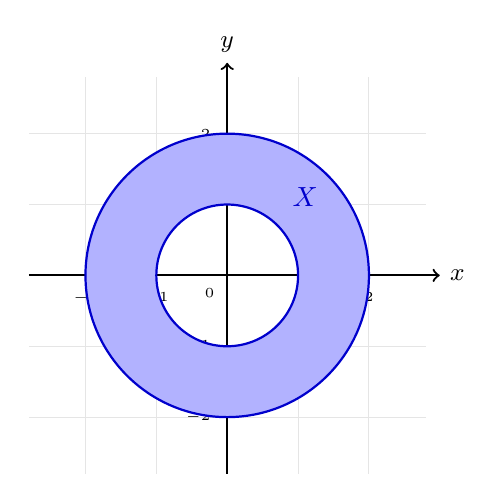
\begin{tikzpicture}[scale=0.9]
            % Grid & Axes
            \draw[gray!20, thin] (-2.8,-2.8) grid (2.8,2.8);
            \draw[->, thick] (-2.8,0) -- (3.0,0) node[right] {\small $x$};
            \draw[->, thick] (0,-2.8) -- (0,3.0) node[above] {\small $y$};
            
            % Ticks
            \foreach \x in {-2,-1,1,2} \draw (\x,0.1) -- (\x,-0.1) node[below] {\tiny $\x$};
            \foreach \y in {-2,-1,1,2} \draw (0.1,\y) -- (-0.1,\y) node[left] {\tiny $\y$};
            \node at (-0.25,-0.25) {\tiny $0$};

            % Shaded Annulus: Outer circle radius 2 minus inner circle radius 1
            \fill[blue!30, even odd rule] (0,0) circle (2cm) (0,0) circle (1cm);
            
            % Solid Boundaries
            \draw[thick, blue!80!black] (0,0) circle (2cm);
            \draw[thick, blue!80!black] (0,0) circle (1cm);
            
            \node[blue!80!black] at (1.1,1.1) {$X$};
        \end{tikzpicture}
        \caption{The set $X$ (Annulus $1 \le r \le 2$)}
    \end{subfigure}\qquad
    % Drawing 2: The Complement X^c
    \begin{subfigure}[b]{0.45\linewidth}
        \centering
        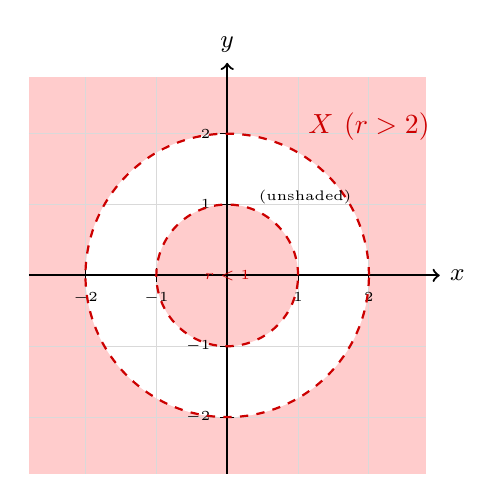
\begin{tikzpicture}[scale=0.9]
            % Outer bounding region shaded
            \fill[red!20] (-2.8,-2.8) rectangle (2.8,2.8);
            
            % Unshade the annulus X
            \fill[white] (0,0) circle (2cm);
            
            % Re-shade the inner core disk r < 1
            \fill[red!20] (0,0) circle (1cm);
            
            % Grid & Axes
            \draw[gray!30, thin] (-2.8,-2.8) grid (2.8,2.8);
            \draw[->, thick] (-2.8,0) -- (3.0,0) node[right] {\small $x$};
            \draw[->, thick] (0,-2.8) -- (0,3.0) node[above] {\small $y$};
            
            % Ticks
            \foreach \x in {-2,-1,1,2} \draw (\x,0.1) -- (\x,-0.1) node[below] {\tiny $\x$};
            \foreach \y in {-2,-1,1,2} \draw (0.1,\y) -- (-0.1,\y) node[left] {\tiny $\y$};
            
            % Dashed boundaries excluded from X^c
            \draw[thick, dashed, red!80!black] (0,0) circle (2cm);
            \draw[thick, dashed, red!80!black] (0,0) circle (1cm);
            
            \node[red!80!black] at (0,0) {\tiny $r < 1$};
            \node[red!80!black] at (2.0,2.1) {$X^{\complement}$ ($r > 2$)};
            \node at (1.1,1.1) {\tiny (unshaded)};
        \end{tikzpicture}
        \caption{The complement $X^{\complement}$ ($r < 1 \cup r > 2$)}
    \end{subfigure}

    \caption{Sketches for Exercise 6.5.}\label{fig:ex_6_5}
\end{figure}
\end{solution}

\begin{solution}\label{sol:6.6}\ref{ex:6.6}
    Ditto.
    
    \begin{figure}[htbp]
    \centering
    % Drawing 1: The set X (y < x^2)
    \begin{subfigure}[b]{0.45\linewidth}
        \centering
        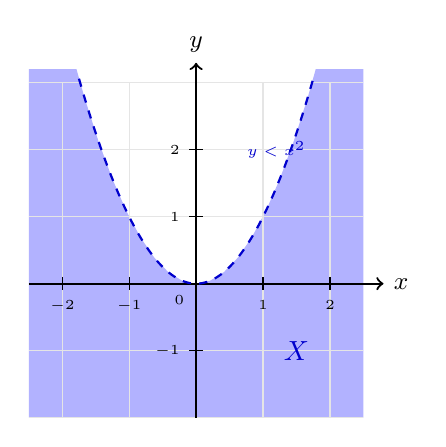
\begin{tikzpicture}[scale=0.85]
            % Bounding area for clip
            \begin{scope}
                \clip (-2.5,-2.0) rectangle (2.5,3.2);
                
                % Fill region below parabola y < x^2
                \fill[blue!30] plot[domain=-2.5:2.5, variable=\x] (\x, {\x*\x}) -- (2.5,-2.0) -- (-2.5,-2.0) -- cycle;
            \end{scope}

            % Grid & Axes
            \draw[gray!20, thin] (-2.5,-2.0) grid (2.5,3.0);
            \draw[->, thick] (-2.5,0) -- (2.8,0) node[right] {\small $x$};
            \draw[->, thick] (0,-2.0) -- (0,3.3) node[above] {\small $y$};
            
            % Ticks
            \foreach \x in {-2,-1,1,2} \draw (\x,0.1) -- (\x,-0.1) node[below] {\tiny $\x$};
            \foreach \y in {-1,1,2} \draw (0.1,\y) -- (-0.1,\y) node[left] {\tiny $\y$};
            \node at (-0.25,-0.25) {\tiny $0$};

            % Dashed parabola boundary y = x^2
            \draw[thick, dashed, blue!80!black, domain=-1.75:1.75, variable=\x, samples=100] plot (\x, {\x*\x});
            
            \node[blue!80!black] at (1.5,-1.0) {$X$};
            \node[blue!80!black, font=\tiny] at (1.2,2.0) {$y < x^2$};
        \end{tikzpicture}
        \caption{The set $X = \{(x,y) \in \mathbb{R}^2 : y < x^2\}$}
    \end{subfigure}\qquad
    % Drawing 2: The Complement X^c (y >= x^2)
    \begin{subfigure}[b]{0.45\linewidth}
        \centering
        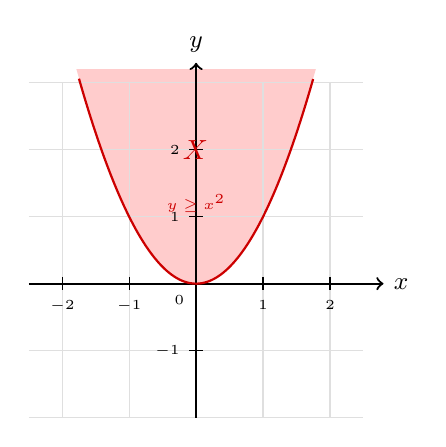
\begin{tikzpicture}[scale=0.85]
            % Bounding area for clip
            \begin{scope}
                \clip (-2.5,-2.0) rectangle (2.5,3.2);
                
                % Fill region on/above parabola y >= x^2
                \fill[red!20] plot[domain=-2.0:2.0, variable=\x] (\x, {\x*\x}) -- (2.5,3.5) -- (-2.5,3.5) -- cycle;
            \end{scope}

            % Grid & Axes
            \draw[gray!25, thin] (-2.5,-2.0) grid (2.5,3.0);
            \draw[->, thick] (-2.5,0) -- (2.8,0) node[right] {\small $x$};
            \draw[->, thick] (0,-2.0) -- (0,3.3) node[above] {\small $y$};
            
            % Ticks
            \foreach \x in {-2,-1,1,2} \draw (\x,0.1) -- (\x,-0.1) node[below] {\tiny $\x$};
            \foreach \y in {-1,1,2} \draw (0.1,\y) -- (-0.1,\y) node[left] {\tiny $\y$};
            \node at (-0.25,-0.25) {\tiny $0$};

            % Solid parabola boundary y = x^2
            \draw[thick, red!80!black, domain=-1.75:1.75, variable=\x, samples=100] plot (\x, {\x*\x});
            
            \node[red!80!black] at (0,2.0) {$X^{\complement}$};
            \node[red!80!black, font=\tiny] at (0,1.2) {$y \ge x^2$};
        \end{tikzpicture}
        \caption{The complement $X^{\complement} = \{(x,y) \in \mathbb{R}^2 : y \ge x^2\}$}
    \end{subfigure}

    \caption{Sketches for Exercise 6.6.}\label{fig:ex_6_6}
\end{figure}
\end{solution}